\chapter{Subsistema de control y presentación}\label{chap:control}

\section{Introducción}

El último de los subsistemas que conforma el sistema de medida digital es
el subsistema de control y presentación. Es el subsistema de más alto nivel
de entre los que integran el sistema por interactuar directamente con el
supervisor. El subsistema de control y presentación está constituido por
los bloques de control y presentación propiamente dichos, tal y como
muestra la \cref{fig:subconpre}. Sin embargo, en la práctica estos dos
bloques se mezclan en una misma entidad indivisible, un software que se
ejecuta en el \pc{} anfitrión en el que se encuentra instalada la tarjeta
de adquisición.  Por ser el software que controla el funcionamiento de la
tarjeta \kpci{} pasa a conocerse como \emph{software de control} en este
documento.

\begin{figure}
	\begin{center}
		\includegraphics{gis-pfc-ch3-01.mps}
	\end{center}
	\caption[Subsistema de control y presentación] {Bloques de control
	y presentación dentro del subsistema de control y presentación.}
	\label{fig:subconpre}
\end{figure}

El subsistema de control y presentación constituye la interfaz entre el
supervisor y el sistema de medida, como tal, es una de sus funciones
proporcionar control sobre el sistema al supervisor: ejecutar las órdenes
administradas por el supervisor y gestionar el funcionamiento del resto de
subsistemas. El bloque de control es el encargado de esta actividad y
desempeña las siguientes tareas:

\begin{itemize}
	\item Iniciar y detener la sesión de adquisición.
	\item Interactuar con los drivers de la tarjeta por medio del
		sistema operativo para controlar parámetros de la sesión de
		adquisición como pueden ser, por ejemplo, puertos de
		entrada, modos de adquisición y terminación, o frecuencia
		de muestreo.
	\item Realizar el mantenimiento de los buffers de memoria. Tarea
		que puede dividirse, o consta a su vez, de dos tareas de
		menor complejidad: dar formato a las muestras almacenadas
		en el o los buffers situados en la memoria interna de la
		tarjeta para su comprensión por parte del ordenador
		anfitrión; trasladar las muestras formateadas adecuadamente
		a la memoria del \pc{} para que de ese modo puedan ser
		manipuladas por el usuario administrador.
\end{itemize}

Por su parte, corresponde al bloque de presentación presentar al supervisor
información de utilidad a partir de la señal digital que procede del
subsistema de adquisición. La información debe mostrarse al supervisor para
que pueda interpretarla. En consecuencia, y sometiendo el diseño de la
aplicación de software al criterio del director del PFC, se concluye en
dotar al bloque de presentación con la capacidad de proporcionar la
siguiente información acerca de la señal:

\begin{itemize}
	\item El valor instantáneo cada 250 ms.
	\item El valor medio en el mismo intervalo de tiempo. Este valor
		debe calcularse a partir de las muestras obtenidas en dicho
		periodo a una frecuencia de muestreo que queda a elección
		del supervisor. Debe ser posible seleccionar la frecuencia
		de muestreo desde el propio software de control.
	\item La forma instantánea de la señal, de un fragmento de una
		duración determinada. Debe ser posible también seleccionar
		la duración del fragmento. Simultáneamente debe
		representarse el espectro en frecuencia del fragmento de
		señal que aparece en pantalla.
\end{itemize}

Este capítulo se ha distribuido en dos apartados. En el primero de los
apartados se describe la herramienta empleada en el desarrollo del software
de control. En el segundo se exponen las conclusiones obtenidas al estudiar
el osciloscopio digital como herramienta de referencia en la representación
gráfica de señales. De ese modo se evita explicar el significado del código
correspondiente al software de control línea por línea, puesto que el
lector puede concebir su propia idea del aspecto que adopta el software en
su estadio definitivo de desarrollo. El ejercicio de reflexión pertinente
conduce a una positiva comprensión del proceso que partiendo del diseño
original concluye en el resultado esperado.

% 				( V )
% ______________________________m\"/m______________________________________
%				  '
% El texto comentado aquí abajo debe trasladarse a otra sección del
% capítulo
% _________________________________________________________________________
%
% Se impone una condición de diseño adicional, el software de control debe
% ser poco exigente a fin de que pueda ser ejecutado en un \pc{} que
% disponga de escasos recursos. Para cumplir con dicha condición se propone
% la siguiente solución: limitar la cantidad de datos diferentes
% presentados por pantalla simultáneamente a uno. De ese modo el usuario
% del software debe elegir en cada momento entre el valor instantáneo, el
% valor medio y la forma de la señal y su espectro en frecuencia, y sólo el
% tipo de dato seleccionado se genera reduciendo el coste de procesado.
% Esta solución puede ampliarse incorporando la posibilidad de deshabilitar
% la representación del espectro o de la forma de la señal.
%
% 				 ,._
%				@",_)6
%				 " "

\section{Herramienta de Adquisición de Datos}


\subsection{Introducción}

\psig{matlab} (\emph{MATrix LABoratory}) es la plataforma seleccionada para
el desarrollo del software de control. Es una plataforma de desarrollo bien
conocida en entornos matemáticos y tecnológicos de uso extendido en
universidades y otros centros educativos y de investigación. Encaja en la
descripción de un kit de desarrollo de software (\sig{sdk}) al estar
compuesto por un entorno de desarrollo integrado (\sig{ide}) con editor,
compilador y depurador; y una colección de módulos y extensiones que en
conjunto se comportan como una interfaz de programación de aplicaciones
(\sig{api}).  \matlab{} se caracteriza por emplear un lenguaje propio, el
lenguaje \psig{m}, enfocado a un uso matemático y que se ha diseñado para
simplificar el manejo de datos agrupados en estructuras matemáticas
complejas como son las matrices y los vectores. Los módulos y herramientas
que se incluyen en el \sig{sdk} contribuyen a ampliar su funcionalidad,
convirtiéndolo en un software potente y completo. Estas herramientas
abstraen al desarrollador de implementar por sí mismo en lenguaje \sig{m}
funciones destinadas a realizar operaciones cotidianas como representar
unos datos por pantalla u obtener la \sig{fft} de un vector. Existen
módulos ---o \emph{toolboxes} como se los conoce en inglés--- mantenidos
por la compañía de software, a los que se suman los diseñados por los
propios usuarios, que abundan en la red, disponibles desde la base de datos
dispuesta para ello por la empresa, con lo que las posibilidades son en la
práctica infinitas.  Además \matlab{} cuenta con dos herramientas
fundamentales, muy ligadas al \sig{sdk}, una es \psig{guide}
(\emph{Graphical User Interface Development Environment}), una herramienta
para el desarrollo de interfaces gráficas de usuario (\psig{gui}); y otra
\emph{Simulink}, herramienta que se emplea para realizar todo tipo de
simulaciones.

Las dos razones principales por las que se utiliza \matlab{} son, por un
lado, las facilidades que aporta en la creación de \gui{} y manejo de
señales digitalizadas; y por otro, y aún más importante si cabe, que
incorpora una herramienta denominada \emph{Data Acquisition Toolbox},
nombre que podría traducirse como Herramienta de Adquisición de Datos, en
lo sucesivo \psig{dat}. La \datx{} es una herramienta compuesta por una
biblioteca y un mecanismo para el intercambio de información, que en
conjunto permiten mediante código de alto nivel interactuar directamente
con dispositivos de características similares a las de la tarjeta de
adquisición \kpci{}, y que es convenientemente compatible con ésta tarjeta.
En otras palabras, puede entenderse la \datx{} como una \sig{api} o
interfaz que proporciona al desarrollador las llamadas necesarias para
interactuar directamente con dispositivos de adquisición al tiempo que
abstrae los mecanismos de más bajo nivel que intervienen en el proceso,
descargando al desarrollador de la responsabilidad de implementarlos por él
mismo. Lo que, al fin y al cabo puede resumirse en que en la \datx{} se
implementa el núcleo de lo que se entiende como bloque de control. Al
programarse el software de control empleando los recursos que proporciona
la \datx{}, la herramienta en sí pasa a ser parte fundamental del
subsistema de control y presentación al prestarse como núcleo del bloque de
control. Cobra pues vital importancia en el sistema de medida. En
consecuencia, resulta adecuado un apartado en el que se introduzca la
herramienta al lector. En primer lugar se describen las distintas entidades
que participan en el funcionamiento de la herramienta, justo después se
recoge un subconjunto de las distintas funciones que la \datx{} pone a
disposición del desarrollador ordenadas siguiendo el mismo orden en el que
son requeridas durante la sesión de adquisición de carácter más básico.


\subsection{Componentes de la herramienta}

Los elementos de \matlab{} que juegan un papel suficientemente importante
en el funcionamiento de la \datx{} son los listados en el
\cref{tab:toolcomp}. El diagrama representado en la \vref{fig:toolcomp}
muestra las interdependencias que existen entre los elementos que aparecen
en dicho cuadro.

\begin{table}
	\centering
	\begin{tabulary}{.9\textwidth}{C L}
		\toprule
		Componente & \multicolumn{1}{c}{Propósito} \\
		\midrule
		Ficheros *.m & Se emplean para automatizar la creación de
		objetos dispositivo, adquirir datos, configurar las
		propiedades del dispositivo y la sesión, y evaluar el
		estado de la adquisición y los recursos.\\
		\midrule
		Máquina virtual de adquisición de datos & Almacena objetos
		dispositivo y sus propiedades, controla el almacenamiento
		de los datos adquiridos y controla la sincronización de
		eventos.\\
		\midrule
		Adaptadores & Son la vía de comunicación entre la máquina
		virtual de adquisición de datos y el hardware por la cual
		se transmiten propiedades, datos y eventos.\\
		\bottomrule
	\end{tabulary}
	\caption[Descripción de los componentes de la \datx{}] {Descripción
	de los componentes de la \datx{}.}
	\label{tab:toolcomp}
\end{table}

\begin{figure}
	\begin{center}
		\includegraphics{gis-pfc-ch3-07.mps}
	\end{center}
	\caption[Elementos que intervienen en el funcionamiento de la
	\datx{}]{Elementos que intervienen en el funcionamiento de la
	\datx{}.}
	\label{fig:toolcomp}
\end{figure}

\subsubsection{Objetos dispositivo}

Los objetos dispositivo permiten el acceso a subsistemas específicos del
hardware. Los objetos dispositivo soportados por la \datx{} son los objetos
de entrada analógica o \emph{analog imput objects} (\psig{ai}), los objetos
de salida analógica o \emph{analog output objects} (\psig{ao}) y los
objetos de entrada/salida digital o \emph{digital I/O objects}
(\psig{dio}).

\begin{figure}
	\begin{center}
		\includegraphics{gis-pfc-ch3-08.mps}
	\end{center}
	\caption[Comunicación entre los subsistemas del hardware y los
	objetos dispositivo]{Grafo que representa la comunicación entre los
	subsistemas del hardware y los objetos dispositivo.}
	\label{fig:subsystemsOO}
\end{figure}


\subsection{La sesión de adquisición de datos}

Una sesión completa de adquisición de datos consiste en cinco pasos:

\begin{enumerate}
	\item Crear el objeto dispositivo.
	\item Añadir canales al objeto dispositivo.
	\item Configurar las propiedades del objeto dispositivo y los
		canales añadidos para controlar el comportamiento de la
		aplicación de adquisición de datos.
	\item Adquirir los datos.
	\item Eliminar el objeto dispositivo.
\end{enumerate}

Cada uno de los pasos se detalla en los puntos subsiguientes.


\subsubsection{Crear el objeto dispositivo}

Para crear un objeto dispositivo, se debe llamar a la función de creación
apropiada o constructor. Como se muestra en el \cref{tab:constructors}, los
constructores reciben un nombre particular en función del tipo de objetos
dispositivo que crean. Para iniciar una sesión de adquisición de datos
analógicos es necesario un comando como el siguiente, \func{analoginput}
\func{(`adaptador', ID)}. Un ejemplo extraído del código fuente de la
aplicación de control muestra cómo hacerlo en el \cref{cod:constructor}.

\begin{table}
	\centering
	\begin{tabular}{l >{\tt}l}
		\toprule
		\multicolumn{1}{c}{Tipo de subsistema} %
		& \multicolumn{1}{c}{\rm Constructor} \\
		\midrule
		Entrada analógica & analoginput(`adaptador', ID); \\
		\midrule
		Salida analógica & analogoutput(`adaptador', ID); \\
		\midrule
		Entrada / Salida digital & digitalio(`adaptador', ID); \\
		\bottomrule
	\end{tabular}
	\caption[Tipos de constructor en función del objeto dispositivo
	creado]{Tipos de función de creación de acuerdo con el tipo
	subsistema al que se orienta el objeto dispositivo creado.}
	\label{tab:constructors}
\end{table}

\begin{lstlisting}[style=displayed, caption={[Método a seguir para crear un
	objeto dispositivo] {Método que evalúa la existencia de un objeto
	dispositivo previo a la llamada de la aplicación, en caso positivo
	lo hereda para su uso posterior, de lo contrario crea uno
	nuevo.}}, label={cod:constructor}]
	set(handles.ai, 'TriggerType', 'Immediate', 'TimerFcn', '', ...
	handles.ai = [];

	if ~isempty(daqfind)
		oldObj = daqfind;

		for i = 1:length(oldObj);
			auxStr = daqhwinfo(oldObj(i));
			auxNum = findstr(' ', auxStr.DeviceName) - 1;
			if strcmp('KPCI-3108', ...
				auxStr.DeviceName(1:auxNum)) && ...
				strcmpi('analoginput', auxStr.SubsystemType);
				handles.ai = oldObj(i);
				warning('El dispositivo esta en uso.');
				break
			end
		end

	end

	if isempty(handles.ai)
		try
			handles.ai = analoginput('keithley');
		catch
			errordlg('No pudo crearse el manejador de dispositivo.');
		end
	end
\end{lstlisting}

El argumento \func{id} es un indicador de dispositivo hardware. Se trata de
un argumento opcional para tarjetas de sonido con \func{id} 0. El argumento
\func{adaptador} requiere el nombre del adaptador de dispositivo hardware.
A continuación, en el \cref{tab:adaptors} se muestra una relación con los
adaptadores de dispositivo cuyo uso es más frecuente y el nombre de
adaptador que debe introducirse como argumento de la llamada a
\func{analoginput}. Por conveniencia se ha añadido Keithley a esta lista.

\begin{table}
	\centering
	\begin{tabular}{l >{\tt\qquad}l}
		\toprule
		\multicolumn{1}{c}{Fabricante de Hardware} %
		& \multicolumn{1}{c}{\rm Nombre de adaptador} \\
		\midrule
		Advantech & advantech \\
		\midrule
		Measurement Computing & mcc \\
		\midrule
		National Instruments & nidaq \\
		\midrule
		Parallel port & parallel \\
		\midrule
		Microsoft Windows & winsound \\
		\midrule
		Keithley Instruments, Inc. & keithley \\
		\bottomrule
	\end{tabular}
	\caption[Valores que puede adoptar el argumento
	\func{adaptador}.]{Valores que puede adoptar el argumento
	\func{adaptador} necesario en la llamada a \func{analoginput}.}
	\label{tab:adaptors}
\end{table}


\subsubsection{Añadiendo canales}

Antes de poder utilizarse, deben añadirse canales al objeto dispositivo.
Para ello, debe emplearse la función \func{addchannel}. Puede pensarse en
un objeto dispositivo como un contenedor de grupos de canales y en los
canales añadidos a un objeto dispositivo como un grupo de canales. Si se
desean añadir dos canales al objeto dispositivo \func{objeto} puede
utilizarse la siguiente llamada \func{cans = addchannel(objeto, 1:2);}.


\subsubsection{Configurando propiedades}

Puede controlarse el comportamiento de una sesión de adquisición de datos o
de una aplicación creada con tal propósito configurando las propiedades de
los objetos dispositivo que intervienen en el proceso de adquisición y de
los canales que dicho objeto contiene. Estas son las reglas principales en
la configuración de propiedades desde la \datx{}.

\begin{itemize}
	\item Los nombres de las propiedades pueden escribirse en
		mayúsculas, minúsculas o combinación de ambas.
	\item Los nombres de las propiedades pueden abreviarse como se
		mostrará a continuación. % Hay que confirmar que se
		% explican las reglas de abreviatura
	\item La función \func{set} aplicada a un objeto dispositivo
		---\func{set(objeto)}--- devuelve todas las propiedades
		configurables de ese objeto. Si se llama a \func{set}
		utilizando como argumento un canal ---\func{set(objeto.}
		\func{.Channel(índice)}---, la función devolverá todas las
		propiedades configurables de dicho canal.
	\item La función \func{get} devuelve todas las propiedades de un
		canal u objeto y el valor que toman en el momento en el que
		se llama a la función si se emplea como único argumento
		dicho canal u objeto ---\func{get(objeto)},
		\func{get(objeto.Channel(índice)}---.  \end{itemize}

Se distinguen dos tipos de propiedades distintas asociadas a los canales
contenidos en un objeto dispositivo.

\begin{description}
	\item[Propiedades comunes] Son aquellas propiedades que se aplican
		todos los canales pertenecientes a un mismo objeto
		dispositivo.
	\item[Propiedades de canal] A diferencia de las propiedades
		comunes, las propiedades de canal pueden configurarse
		individualmente por canal.
\end{description}

Dentro de las propiedades comunes de los canales existen las
\emph{propiedades básicas}, que se aplican a todos los subsistemas de un
determinado tipo (\textsc{ai, ao, dio}); y \emph{propiedades específicas de
dispositivo} aplicables únicamente al hardware específico que se está
empleando.

Existen tres formas de configurar u obtener el valor de una propiedad:
utilizando las funciones \func{set} y \func{get}; empleando la notación de
punto; o recurriendo a los nombres indexados.

\begin{itemize}
	\item La sintaxis de las funciones \func{get} y \func{set} es
		similar a la empleada en la herramienta de \matlab{}
		\emph{Handle Graphics}.

		\begin{lstlisting}[gobble=16]
			out = get(objeto, `SampleRate');
			set(objeto, `SampleRate', 11025)
		\end{lstlisting}

	\item La notación de punto se emplea del siguiente modo:

		\begin{lstlisting}[gobble=16]
			out = objeto.SampleRate;
% 			objeto.SampleRate = 11025;
		\end{lstlisting}

	\item Por último, los nombres indexados permiten asociar un nombre
		descriptivo a cada canal. Por ejemplo para asociar el
		nombre \func{Can1} con el primer canal contenido en
		\func{objeto} debe procederse como se enuncia a
		continuación.

		\begin{lstlisting}[gobble=16]
			set(objeto.Channel(1), `ChannelName', `Can1');
			out = objeto.Can1.UnitsRange;
			objeto.Can1.UnitsRange = [0, 10];
		\end{lstlisting}

\end{itemize}


\subsubsection{Adquisición de datos}

La adquisición de datos puede dividirse en tres tareas básicas: iniciar el
objeto dispositivo; registrar datos y detener el objeto dispositivo.

La función que se utiliza para iniciar un objeto dispositivo es la función
\func{start}, p.e. para iniciar el objeto dispositivo \func{objeto} habría
que llamar a la función de esta forma \func{start(objeto)}. Tras iniciar un
objeto su propiedad \textsf{Running} pasa de manera automática al valor
\textsf{On}.

No obstante haber iniciado el dispositivo, este no empieza a registrar
datos hasta que no ocurre un trigger o disparo. Hay diversos tipos de
trigger, en el \vref{tab:triggers} se muestran aquellos soportados por
todos los dispositivos. Tras un trigger el dispositivo hardware inicia la
adquisición de datos y la propiedad \textsf{Logging} del objeto dispositivo
asociado conmuta al estado \textsf{On}.

\begin{table}
	\centering
	\begin{tabulary}{.9\linewidth}{>{\sf}c L}
		\toprule
		{\rm Tipo de disparo} & \multicolumn{1}{c}{Descripción} \\
		\midrule
		Inmediato & El disparo ocurre justo después de la llamada a
		\func{start}. Este es el tipo de trigger predeterminado. \\
		\midrule
		Manual & El disparo ocurre después de llamar manualmente a
		la función \func{trigger}. \\
		\midrule
		Software & El disparo sucede cuando se detecta una señal
		que satisface una determinada condición especificada de
		antemano. El objeto dispositivo debe disponer de más de un
		canal que hará las veces de la señal de disparo. Debe
		especificarse, como es obvio, que canal actúa como fuente
		del disparo. \\
		\midrule
		Reloj interno & Por añadidura, la \kpci{} cuenta con la
		posibilidad de recibir el disparo de la fuente de reloj
		interna. \\
		\bottomrule
	\end{tabulary}
	\caption[Tipos de disparo soportados por el hardware compatible con
	\matlab{}]{Tipos de disparo soportados por el hardware compatible
	con \matlab{} y una breve descripción de los mismos.}
	\label{tab:triggers}
\end{table}

Por último, existen tres causas por las que un objeto dispositivo puede
detenerse: \matlab{} detiene un objeto dispositivo iniciado una vez
obtenidos los datos precisados por el usuario; al ocurrir un error de
tiempo de ejecución en relación con la actividad de un objeto dispositivo
éste es detenido también; y tan sólo resta el método manual, que consiste
en llamar a la función \func{stop}, por ejemplo \func{stop(objeto)}.

Como se ha mencionado la máquina virtual de adquisición de datos registra y
controla los datos que extrae de un objeto dispositivo. Un usuario puede
acceder a esos datos de dos formas diferentes:

\begin{itemize}
	\item La primera de ellas se conoce como previsualizar los datos.
		Se emplea con ese propósito la función \func{peekdata}. Si,
		por ejemplo, se quisiese previsualizar 1000 muestras
		obtenidas con el objeto dispositivo \func{objeto}, la
		llamada a \func{peekdata} sería la siguiente: \func{out =
		peekdata(objeto, 1000);}. La función \func{peekdata}
		devuelve el control a \matlab{} de inmediato y no elimina
		los datos previsualizados de la máquina virtual de
		adquisición.
	\item En cualquier momento tras adquirir datos mediante un objeto
		dispositivo estos pueden extraerse de la máquina virtual de
		adquisición mediante la función \func{getdata}. Partiendo
		del ejemplo anterior, si se desea extraer 1000 muestras
		procedentes del objeto dispositivo \func{objeto}, esta es
		la llamada adecuada \func{out = getdata(objeto, 1000);}. Al
		contrario que la función \func{peekdata}, \func{getdata} no
		devuelve el control a \matlab{} hasta haber extraído todas
		las muestras solicitadas. Es evidente que las muestras
		extraídas dejarán de estar disponibles en la máquina
		virtual de adquisición.
\end{itemize}

Es importante señalar que en cualquiera de los procedimientos descritos
intentar acceder a más datos de los obtenidos en un determinado momento
causará un error que detendrá el funcionamiento del objeto dispositivo.


\subsubsection{Eventos y Callbacks}

Puede decirse que un evento sucede en un determinado instante después de
que una cierta condición se cumple. A menos que ocurra un error, en todas
las sesiones de adquisición de datos debe producirse un evento de inicio,
uno de disparo y uno de parada. Puede accederse a la información que
transporta un evento mediante la propiedad \textsf{EventLog}:

\begin{lstlisting}
	Events = ai.EventLog;
	EventTypes = {Events.Types}
	EventTypes =
		`Start'    `Trigger'	`Stop'
\end{lstlisting}

Cuando se produce un evento, puede ejecutarse una función de
\emph{callback}. Es posible seleccionar una función para un callback
especificando como valor de la propiedad asociada a dicho callback el
nombre de la función (si ésta se encuentra en el mismo fichero *.m que
contiene el código que ejecuta la aplicación que realiza la adquisición de
datos), o el nombre del fichero *.m con el código de la función. Así mismo,
pueden pasarse argumentos de entrada a la función de callback asignándolos
a la mencionada propiedad.

Por ejemplo, los siguientes comandos configuran \func{objeto} de forma que
la función \func{datadqcallback} se ejecute desde el fichero cuyo nombre
está compuesto por una raíz idéntica al nombre de la función y con
extensión *.m, cuando se produzca un evento de trigger o de parada durante
la actividad del objeto dispositivo. Además se pasa como argumento de la
función el valor de la propiedad \textsf{Running} de \func{objeto} en el
momento del callback.

\begin{lstlisting}
	set(objeto, `TriggerFcn', @datadqcallback, objeto.Running)
	set(objeto, `StopFcn', @datadqcallback, objeto.Running)
\end{lstlisting}

Un segundo ejemplo, este extraído del código fuente de la aplicación de
control muestra como pasar argumentos a la función de callback y cuál es la
sintaxis de la definición de la misma en el \cref{cod:callback}.

\begin{lstlisting}[style=displayed, caption={[Configuración de
	\emph{callback}]{Configuración de \emph{callback} para responder a
	eventos en la sesión de muestreo, la función de \emph{callback}
	recibe un argumento.}}, label={cod:callback}]
	set(handles.ai, 'TriggerType', 'Immediate', 'TimerFcn', '', ...
		'SamplesAcquiredFcn', {@localDaqCallback, gcbo});

				[...]

	function localDaqCallback(obj, event, hObject)
		handles = guidata(hObject);
		EventType = event.Type;

		switch lower(EventType)
			case 'samplesacquired'

				[...]

			case 'timer'

				[...]

		end
\end{lstlisting}

\subsubsection{Suprimiendo y borrando las trazas de los objetos dispositivo}

La función \func{delete} elimina el objeto dispositivo especificado de la
máquina virtual de adquisición, pero no del espacio de trabajo (espacio
reservado a las variables de trabajo) de \matlab{},
---\func{delete(objeto)}---. Tras una llamada semejante \func{objeto} sigue
apareciendo en el espacio de trabajo de \matlab{}, pero se trata de un
objeto inválido desde el momento en el que deja de encontrarse ligado al
hardware. Deben suprimirse los objetos dispositivo faltos de validez con el
comando \func{clear}, p.e., \func{clear objeto}.

Si se suprime un objeto dispositivo del espacio de trabajo de \matlab{} no
deja de existir en la máquina virtual. Para poder recuperar objetos
borrados accidentalmente puede utilizarse la función \func{daqfind}.

\begin{lstlisting}
	out = daqfind;	ai = out(1);
\end{lstlisting}


\section{Diseño conceptual del software}

\matlab{} y la \datx{} simplifican en gran medida la tarea de implementar
el bloque de control y la interfaz gráfica de usuario, por tanto, el último
reto importante que debe afrontarse en el desarrollo del software de
control es programar el mecanismo mediante el cual ha de representarse la
señal en pantalla. Es sencillo mostrar por pantalla datos numéricos o
representar la \sig{fft} de una señal, gracias a las utilidades de que
dispone \matlab{}, representar una señal en <<tiempo real>> es algo más
complejo. Al fijar los objetivos del \sig{pfc} se especifica que debe poder
utilizarse el sistema de medida para visualizar señales como si se tratase
de un osciloscopio digital. La principal complicación que existe al
programar un osciloscopio digital en software radica en definir las metas
de programación y no en escribir el código. Esto sólo puede lograrse tras
estudiar en profundidad el modelo, después de comprender perfectamente su
comportamiento y de ese modo poder traducir sus principales rasgos de
conducta en metas sencillas. En este apartado se exponen brevemente las
conclusiones extraídas tras estudiar el osciloscopio digital como modelo
para el software de control.


\subsection{Osciloscopios digitales}

Un osciloscopio digital es una herramienta que se emplea para visualizar
señales. Es el sucesor de instrumentos de medida como el osciloscopio
analógico y el oscilógrafo. A diferencia de estos aparatos de carácter
analógico, un osciloscopio digital debe muestrear parte de la señal,
procesar la señal digital resultante y almacenar las muestras en memoria
antes de poder representar en la pantalla una última versión de la señal
obtenida por interpolación de las muestras. Tratar de representar cada
muestra según se origina en el conversor analógico digital trae consigo un
conjunto de complicaciones difíciles de salvar, sin mencionar que ha de
sacrificarse parte del rendimiento de muestreo, lo que significa que se
pierde la capacidad de trabajar con señales de gran ancho de banda en
ausencia de aliasing. El tratamiento de la señal digital conlleva, sin
embargo, una serie de desventajas, de entre las cuales cabe destacar la
aparición de un retardo entre la señal que registra la sonda del
osciloscopio y la señal mostrada por pantalla. El retardo, de ser demasiado
alto, puede entorpecer el uso del osciloscopio, lo cual no debe ocurrir en
ningún caso, por tanto, debe mantenerse por debajo de un nivel de umbral.
El nivel de umbral se elige de forma que por debajo del mismo el retardo no
puede ser percibido por el ojo humano, lo que a efectos prácticos es lo
mismo que un retardo inexistente. El control del retardo condiciona el
funcionamiento del osciloscopio, limitando la cantidad de muestras que
pueden almacenarse en memoria antes de cada nuevo ciclo.

Los osciloscopios analógicos emplean un tubo de rayos catódicos y un
monitor de fósforo para generar una imagen de la señal. El cursor que el
tubo dibuja en el monitor lo va barriendo de izquierda a derecha con
periodicidad, y su posición vertical refleja a cada momento el valor de
tensión de la señal eléctrica que entra al osciloscopio. El monitor
preserva durante breves instantes una traza del cursor y así se forma la
imagen que representa a la señal.

En la actualidad los osciloscopios analógicos están siendo desplazados en
su uso por los osciloscopios digitales. El procedimiento que sigue un
osciloscopio digital para representar señales es completamente diferente al
que siguen los osciloscopios analógicos. Constantemente el osciloscopio
digitaliza la señal en seguimiento, procesa la señal digital resultante y
la almacena en memoria. Cada cierto \emph{periodo de refresco} el
osciloscopio muestra por pantalla una representación de los datos que
previamente ha almacenado durante ese mismo periodo. Mientras se recogen
datos para una nueva imagen se mantienen en pantalla los datos
correspondientes al periodo anterior. La velocidad con la que se suceden
las imágenes en el monitor del osciloscopio hace que se produzca la
sensación de movimiento, y de ese modo la representación responde a las
variaciones que se producen en la señal. Esto permite observar los eventos
que se producen en la señal en determinadas situaciones, como por ejemplo:
al accionar un potenciómetro que forma parte de un circuito que está siendo
analizado, al cambiar la configuración de un generador de señales para que
genere una señal diferente a la que suministraba unos instantes antes, o
simplemente al conectar la alimentación.

El periodo de refresco no es fijo, de lo contrario los datos mostrados en
el monitor del osciloscopio aparecerían en exceso comprimidos o expandidos
en función de la frecuencia de la señal monitorizada. Puede configurarse el
periodo de muestreo para que adopte un valor de entre un rango de valores
predeterminados. Debe notarse que al ser posible modificar el valor del
periodo de refresco existe la posibilidad de que, en efecto, éste adopte un
valor alto. Ésto haría que el retardo que se produce en la sucesión de
imágenes aumentase, limitando la capacidad de la representación de seguir
los cambios que afectan a la señal. Para impedir que ésto ocurra los
osciloscopios digitales implementan un mecanismo por el cual una señal se
representa de uno u otro modo en función del valor que toma el periodo de
refresco.


\subsection{Modos de representación en los osciloscopios digitales}\label{subsec:repmodes}

Los osciloscopios digitales tienen la capacidad de representar una señal de
formas diferentes. Cada forma de representar la señal se conoce en este
documento como \emph{modo de representación}. Habitualmente los
osciloscopios digitales cuentan al menos con dos modos de representación.
Estos dos modos son, tal y como han sido bautizados aquí, el \emph{modo
disparado} y el \emph{modo continuo}. Los modos de representación continuo
y disparado forman parte de la solución que los osciloscopios digitales
adoptan para combatir la situación hipotética en la que un excesivo retardo
entre cuadros pudiese complicar el seguimiento de la señal.

Para evitar las consecuencias de un retardo alto, un osciloscopio digital
conmuta al modo de representación continuo cuando el periodo de refresco
supera los 200 ms, el resto del tiempo permanece en el modo de
representación disparado. % Para remediar el retardo, un osciloscopio
% digital conmuta al modo de representación continuo cuando el periodo de
% refresco supera los 200 ms, el resto del tiempo permanece en el modo de
% representación disparado.

Para evitar las limitaciones que el modo de representación disparado
presenta en configuraciones en las que el periodo de refresco toma un valor
elevado, un osciloscopio conmuta al modo de representación continuo en el
caso en el que el periodo de refresco supere los 200 ms. Habitualmente el
osciloscopio digital opera en el modo de representación disparado, que es
el modo que responde a la descripción funcional que se ha hecho de los
osciloscopios digitales en este apartado.


\subsubsection{Criterios para la selección del modo}

Para evitar que en determinadas configuraciones del eje temporal del
osciloscopio el retardo sea excesivo, la mayoría de estos dispositivos
implementan dos modos de funcionamiento: el modo convencional que se aplica
en situaciones en las que el retardo no se considera importante; y una
especie de modo continuo. Existen dos criterios que se siguen de manera
habitual para diferenciar en que momento es más apropiado el uso de uno u
otro modo.


\subparagraph{Criterio de animación}

El primer criterio evalúa el correcto funcionamiento del modo convencional.
El modo convencional de representación en un osciloscopio requiere que la
cantidad de imágenes que salen por pantalla cada segundo sea lo suficiente
grande como para que se simule el movimiento. Por tanto para satisfacer el
primer criterio, la tasa de refresco del monitor del osciloscopio debe
superar las veintiséis imágenes por segundo o encontrarse alrededor de esta
cifra.


\subparagraph{Criterio de disparo}

El segundo criterio está relacionado con la función de disparo que se da en
el modo convencional de representación. Para poder efectuar correctamente
el disparo sobre señales de baja frecuencia, al generar cada imagen el
osciloscopio debe haber registrado al menos un ciclo de la señal
pertinente\footnote{En la práctica se necesita algo más de un ciclo de una
señal para poder garantizar el correcto disparo de ésta. Sin embargo, es
común conseguir disparar una señal aunque la configuración del eje de
tiempos del osciloscopio permita sólo obtener una fracción del ciclo
completo de esa señal durante la realización de cada imagen.}. Lo cual
reduce la tasa mínima de refresco a la frecuencia de la señal más lenta que
se desee representar de forma correcta en el modo convencional de
representación del osciloscopio.

Como puede verse el segundo criterio es más restrictivo pues depende de la
frecuencia de la señal y ésta puede ser en efecto inferior a un hercio, es
por ello que se emplea habitualmente. Siendo así, la tasa de refresco
mínima que se permite en el modo convencional en la gran mayoría de
dispositivos y que se ha adoptado para el software de control, es de cinco
imágenes por segundo (5 Hz). Cuando se configura un osciloscopio en el modo
convencional para que trabaje a esta tasa de refresco es habitual poder
visualizar señales de frecuencia cercana a 1 Hz, sin embargo la
representación se optimiza para configuraciones en las que el osciloscopio
muestra, al menos, veinticinco imágenes por segundo, lo cual es apropiado
para señales con una frecuencia mínima de 50 Hz. Si la configuración del
eje de tiempos del osciloscopio obligara al dispositivo a trabajar con una
frecuencia de refresco inferior a la especificada, automáticamente conmuta
para funcionar en el modo continuo.


\subsubsection{Modos de representación}

Una vez visto cual es la frecuencia umbral a la que el dispositivo conmuta
entre los dos modos, debe explicarse que diferencia un modo de
funcionamiento de otro. Para ello se expone a continuación cuales son los
fundamentos de uno y otro modo.


\subparagraph{Modo continuo}

La representación en \emph{modo continuo} es, por decirlo así,
ininterrumpida. La imagen de la señal de interés se desplaza de derecha
izquierda a medida que transcurre el tiempo. Para lograr este efecto se
aumenta la frecuencia de refresco a expensas de que, como es sabido, el
fragmento de señal obtenido para cada imagen no puede cubrir la pantalla al
completo. Ocurre así por que la frecuencia de refresco es muy alta para el
eje temporal, que en este caso representa un periodo tiempo relativamente
alto. Por consiguiente, en el intervalo en el que una imagen de la señal da
paso a la siguiente en la ventana del osciloscopio, no transcurre el tiempo
suficiente como para captar un fragmento de señal de duración igual a la
abarcada por el eje de tiempos.

Las figuras \cref{fig:freesignalcont,fig:modconti} muestran con detalle
estos aspectos del modo de representación continuo. En la
\cref{fig:freesignalcont} aparece la señal que entra en el osciloscopio, se
muestran además unas marcas de tiempo que indican los instantes en los que
la imagen que muestra el osciloscopio cambia\footnote{Se ha considerado el
\emph{periodo de refresco} de la ventana del osciloscopio igual a la suma
de la \emph{ventana de adquisición} y un \emph{periodo de inactividad} en
la adquisición ocupado por el procesado de las muestras. La ventana de
adquisición es equivalente a la cantidad de tiempo que el sistema necesita
para adquirir un fragmento de señal suficiente para cubrir una porción del
eje de tiempos (en el caso del modo de funcionamiento continuo) o para
cubrir el eje de tiempos por completo más las muestras de descarte (en el
modo disparado). El periodo de inactividad es igual al tiempo requerido
para procesar el fragmento de señal adquirido en el espacio de una ventana
de adquisición.}. La \cref{fig:modconti} muestra cual es el aspecto del
osciloscopio en dos instantes posteriores al instante inicial en el que
empieza a monitorizarse la señal.

\begin{figure}
	\begin{center}
		\includegraphics{gis-pfc-ch3-04.mps}
	\end{center}
	\caption[Fragmentos de señal ordenados según el orden en el que
	llegan al sistema]{Fragmentos de señal ordenados según el orden en
	el que llegan al sistema. Cada instante marcado se encuentra
	separado de los adyacentes por un periodo de refresco. Debe
	recordarse que el modo de funcionamiento continuo se emplea en la
	monitorización de señales lentas, por lo que el periodo de
	inactividad es en este caso despreciable frente a la duración de la
	ventana de adquisición.}
	\label{fig:freesignalcont}
\end{figure}

\begin{figure}
	\begin{center}
		\includegraphics{gis-pfc-ch3-05.mps}
	\end{center}
	\caption[Dos líneas de prueba]{Dos líneas de texto de prueba para
	comprobar como cambia la estructura del documento si lo comprimo un
	poquito.}
% 	\caption[<++>]<++>{}<++>
% 	\caption[Modo de funcionamiento continuo]{Puede observarse como la
% 	llegada de un nuevo fragmento de señal al sistema en el instante
% 	$t_2$ desplaza el fragmento previamente representado en la ventana
% 	del osciloscopio una periodo de refresco a la derecha.}
	\label{fig:modconti}
\end{figure}

En el instante $t_1$ el fragmento de señal que se ha digitalizado aparece
en el extremo derecho de la representación, el resto se deja en blanco. En
cada nuevo fotograma se desplazan los fragmentos de señal representados
hasta el momento el suficiente espacio hacia la izquierda como para
incorporar un nuevo fragmento de señal. Así la porción de señal
representada aumenta cada vez más hasta que el extremo izquierdo de la
figura alcanza el margen izquierdo de la ventana del osciloscopio. Cuando
esto ocurre, empieza un desplazamiento cíclico, al incorporar un nuevo
fragmento de señal a la derecha se retira un fragmento de la misma
proporción temporal al otro extremo. Este fenómeno bien puede observarse en
la \cref{fig:modcontii}, en el ejemplo el eje temporal es equivalente a
cinco ventanas de adquisición, la llegada de un sexto fragmento de señal al
sistema conduce al inicio de la representación cíclica.

\begin{figure}
	\begin{center}
		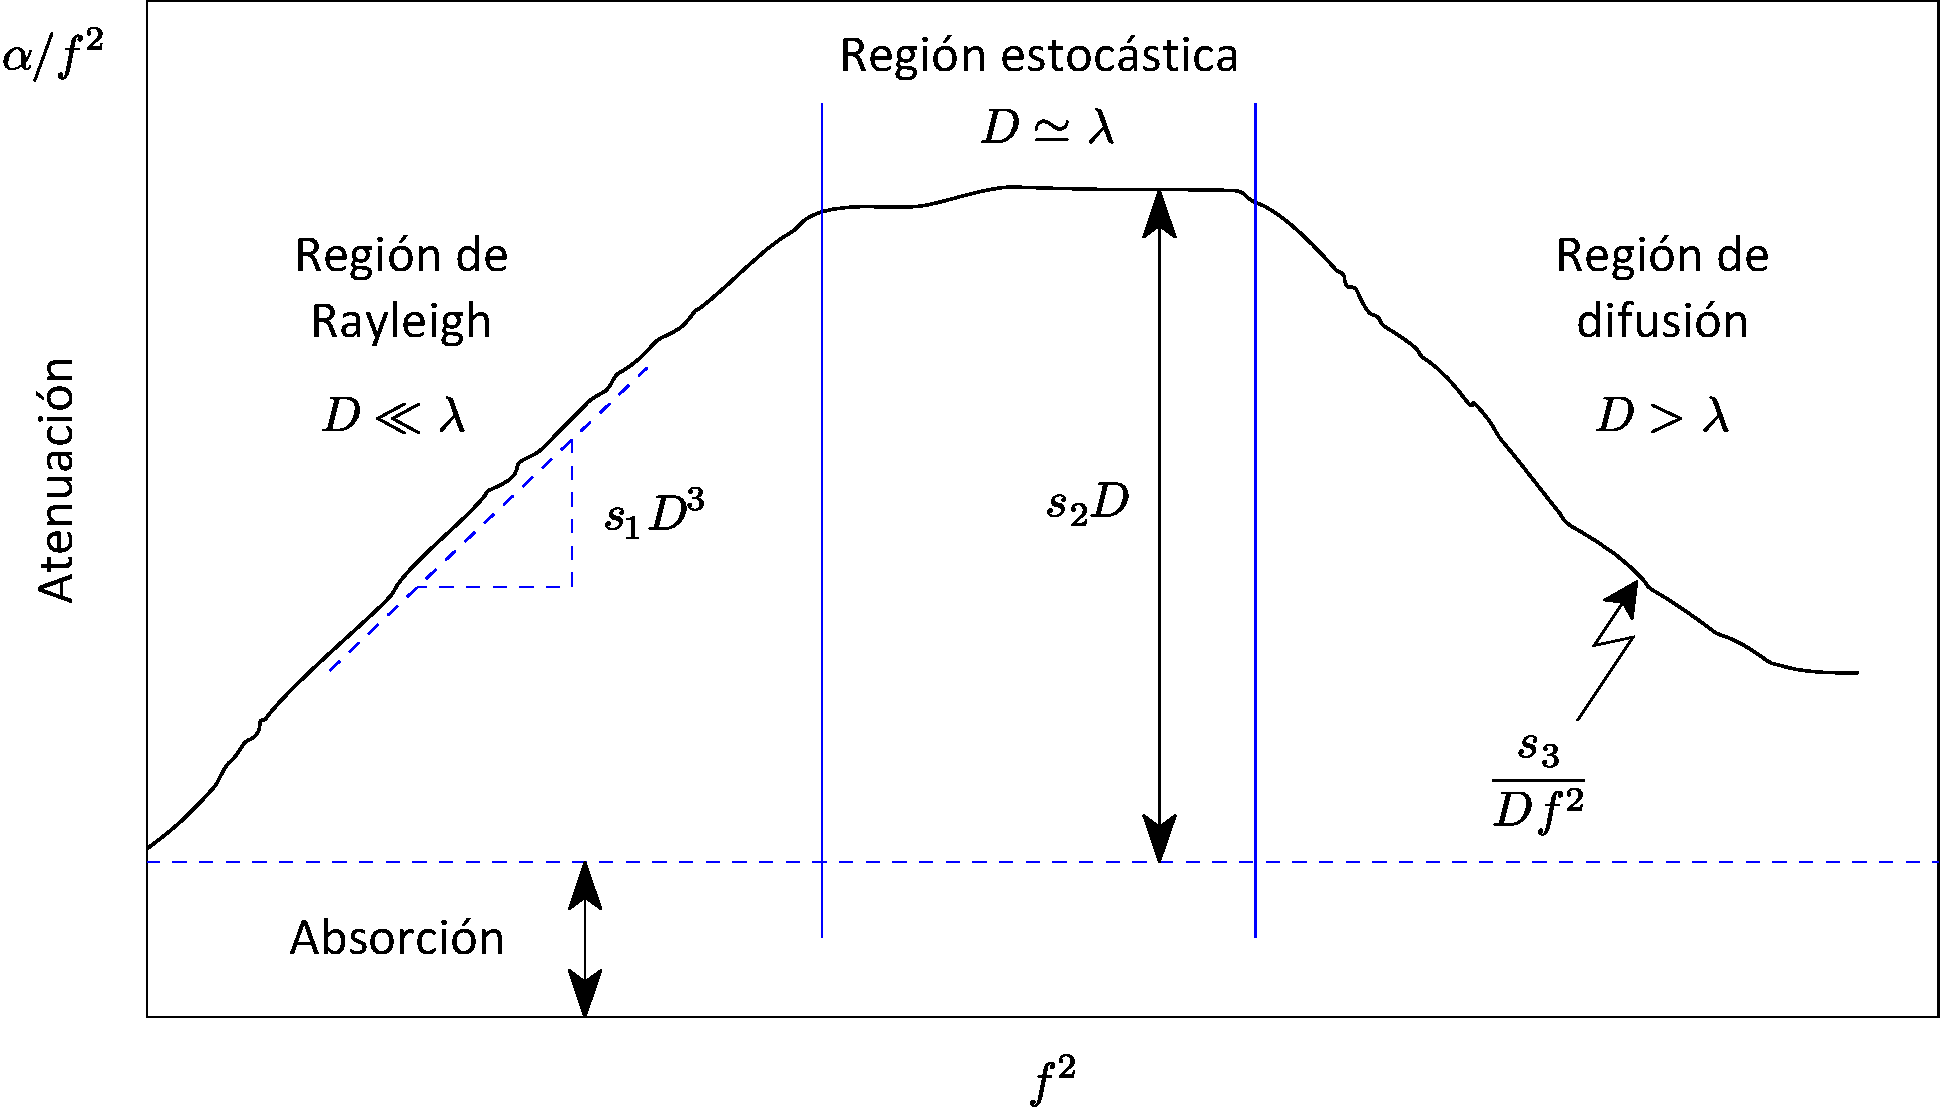
\includegraphics{gis-pfc-ch3-06.mps}
	\end{center}
	\caption[Dos líneas de prueba]{Dos líneas de texto de prueba para
	comprobar como cambia la estructura del documento si lo comprimo un
	poquito.}
% 	\caption[Modo de funcionamiento continuo]{La ventana temporal %
% 	tiene, en este ejemplo, una duración de cinco ventanas de %
% 	adquisición. Al llegar al sistema el sexto fragmento de señal, la %
% 	representación avanza a la derecha retirándose el primer fragmento %
% 	representado para dar cabida al fragmento obtenido recientemente.}
	\label{fig:modcontii}
\end{figure}

La alta tasa con la que aparecen las imágenes por pantalla garantizan que
la representación siga casi en tiempo real ---por lo menos así lo percibe
el ojo humano--- a la señal verdadera. Debe notarse, no obstante, que este
método de representación no es adecuado para señales de alta frecuencia
pues aunque el eje temporal abarque un tiempo mayor, la dimensión del
monitor obviamente no varía y las señales de alta frecuencia aparecerán en
exceso comprimidas.


\subparagraph{Modo convencional}

El \emph{modo convencional} de representación es algo más complicado. La
representación convencional basa su funcionamiento en imágenes que muestran
fragmentos de señal que cubren la dimensión temporal de la ventana del
osciloscopio y que se suceden unas a otras con presteza. La idea que
persigue este método es la de conseguir algo semejante a una película de la
señal. Para ello, no es sólo suficiente con que aparezcan muchas imágenes
por segundo en el monitor del osciloscopio, esas imágenes deben estar de
algún modo relacionadas entre sí. Si las imágenes que aparecen en el
monitor son de forma consecutiva muy diferentes es probable que no pueda
discernirse nada claro, y en ese caso de nada vale la representación.

Ahí es donde entra en juego el procesado y la función de disparo de un
osciloscopio digital. Cuando un fragmento suficientemente largo como para
cubrir la ventana de representación se digitaliza y se almacena en memoria,
empieza el procesado digital del mismo. El propósito del procesado es, ente
otras cosas, eliminar las posible componente en continua, averiguar
información adicional de la señal en la medida de lo posible, como p. ej.
su valor de pico a pico, o implementar la función de disparo. La función de
disparo del osciloscopio persigue alinear los ejes verticales de la ventana
donde se representa con los cruces de la señal con respecto a un
determinado valor de umbral que puede ser configurado por el usuario. La
idea es alinear al menos el cruce más centrado de cada fragmento de señal
con el eje de abscisas que corta en dos mitades la ventana. Para
conseguirlo, durante el procesado se detectan todos los cortes de la señal
con el umbral y después se desplaza el fragmento de señal para que el corte
más centrado case con el eje de abscisas. Si la señal es periódica las
variaciones entre un fotograma y el siguiente serán mínimas, puesto que
ambos estarán alineados, y se simulará con éxito el movimiento.

No obstante, la necesidad de desplazar el fragmento de señal que va a
representarse presenta un inconveniente importante. Para poder desplazar el
fragmento de señal y que se cubra completamente la ventana del osciloscopio
su duración debe ser superior al tiempo reflejado en el eje de tiempos de
la ventana. De lo contrario la señal aparecerá truncada, se mostrará un
espacio en blanco y con una tasa de refresco alta la visualización será
confusa. Desplazar fragmentos de señal implica dos cosas: por un lado el
osciloscopio debe esperar más tiempo para refrescar la pantalla, es decir,
se reduce la tasa de refresco para una misma configuración del eje de
tiempos; y por otro, al tener para representar un fragmento de señal de
mayor duración que la reflejada por el eje temporal de la ventana parte del
fragmento queda ahora fuera de la representación.

Este inconveniente se ve paliado por el hecho de que el modo convencional
contempla en principio trabajar con señales de alta frecuencia. Estas
señales cambian de forma tan rápida que de no ser por el disparo sería
imposible observar los cambios. Por otro lado puede seleccionarse que
información que se muestra por pantalla accionando un control de
desplazamiento temporal o modificando el valor de umbral de disparo y,
generalmente, la pérdida de información a causa del disparo no es
significativa.

Para terminar este apartado se han adjuntado las
\cref{fig:freesignaltrig,fig:modtrig} que muestran los distintos aspectos
del modo disparado de funcionamiento del osciloscopio que se han expuesto
aquí. La \cref{fig:freesignaltrig} muestra la señal que entra al sistema,
se han marcado los instantes en los que se suceden los eventos más
relevantes en la representación de un fragmento de señal. También se
muestran el nivel de umbral y la porción de fragmento de señal que coincide
con las muestras descartadas. Otra figura, la \cref{fig:modtrig} muestra
cual es el resultado de representar el fragmento de señal en la ventana del
osciloscopio.

\begin{figure}
	\begin{center}
		\includegraphics{gis-pfc-ch3-02.mps}
	\end{center}
	\caption[Fragmento de señal adquirido por el osciloscopio en el
	espacio de una ventana de adquisición]{Fragmento de señal adquirido
	por el osciloscopio en el espacio de una ventana de adquisición. En
	esta figura se ha representado también la duración de la ventana
	temporal del osciloscopio, pudiendo observarse que información se
	descarta. También se indica el instante en el que se inicia una
	nueva instancia del proceso de adquisición, de lo que puede
	deducirse que información se pierde entre instancias. Los cortes de
	la señal con el nivel de disparo también están representados.}
	\label{fig:freesignaltrig}
\end{figure}

\begin{figure}
	\begin{center}
		\includegraphics{gis-pfc-ch3-03.mps}
	\end{center}
	\caption[Modo de funcionamiento disparado]{Modo de funcionamiento
	disparado. La representación se centra en el corte central (veáse
	la \vref{fig:freesignaltrig}).}
	\label{fig:modtrig}
\end{figure}
